\label{subsub:expOnlineBenchmarks}
\begin{figure}
    \centering
    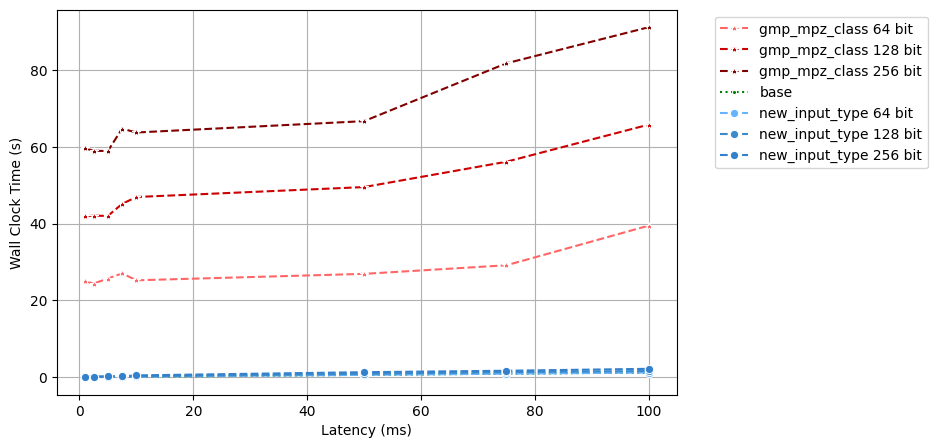
\includegraphics[width=0.8\textwidth]{plots/plots/online/wct_latency_read_online.png}
    \caption{Online: Reading for increasing latency, constant bandwidth, and constant number of elements retrieved.
    The green curve is the base implementation by Vadapalli et al. 
    Red curves represent \textit{gmp\_mpz\_class}.
    The darker the red, the greater the entry size.
    \textit{128 bit}, for example, implies entry sizes of up to 128 bit.
    The blue curve represents \textit{new\_input\_type}.
    }
    \label{fig:readIncLatencyOnline}
\end{figure}

\begin{figure}
    \centering 
    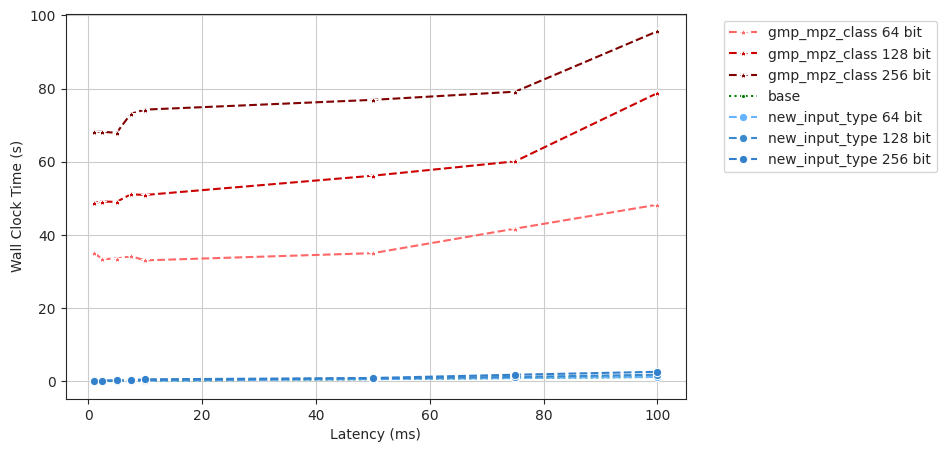
\includegraphics[width=0.8\textwidth]{plots/plots/online/wct_latency_update_online.png}
    \caption{Online: Updating for increasing latency, constant bandwidth, and constant number of elements updated.
    The green curve is the base implementation by Vadapalli et al. 
    Red curves represent \textit{gmp\_mpz\_class}.
    The darker the red, the greater the entry size.
    \textit{128 bit}, for example, implies entry sizes of up to 128 bit.
    The blue curve represents \textit{new\_input\_type}.
    }
    \label{fig:updIncLatencyOnline}
\end{figure}

\ref{fig:readIncLatencyOnline} and \ref{fig:updIncLatencyOnline} show similar results as in the preprocessing phase.
For both reading and updating \textit{gmp\_mpz\_class} is slower than \textit{new\_input\_type} and \textit{base}.
\textit{new\_input\_type} performs nearly as well as \textit{base}.

Recall the idea of \textit{new\_input\_type} where independent reads or updates are executed in parallel (\ref{sub:PossibilityLargerRegisterType}).
Therefore, especially when multithreading, \textit{new\_input\_type} has nearly no performance overhead comparing it with \textit{base}.
This changes, however, for decreasing bandwidth.
Again, for reading (\ref{fig:readIncLatencyOnline}) and updating (\ref{fig:updIncLatencyOnline}) \textit{new\_input\_type} slows down once the bandwidth drops.
The same reasons mentioned above apply:
\textit{new\_input\_type} sends fewer messages compared to \textit{gmp\_mpz\_class} on the same bit size as, again, \textit{gmp\_mpz\_class} needs to send at least two messages for each message \textit{new\_input\_type} sends.
The larger number of sent messages for \textit{gmp\_mpz\_class} is plotted for reading (\ref{fig:readMsgSentOnline}) and updating (\ref{fig:updMsgSentOnline}).
Also, messages in \textit{gmp\_mpz\_class} are smaller on average since, again, using a buffer is not possible.
Messages need to be sent directly.

The algorithm for reading and writing has not been fundamentally changed. 
Therefore, the number of sent messages keeps its linear behavior as the number of read or updated elements increases. 
Only the gradient and the starting point varies depending on the chosen approach.

Ultimately, the online phase shows a similar pattern as the preprocessing phase: 
\textit{gmp\_mpz\_class} is slower on average than \textit{new\_input\_type} on the same bit sizes. 
\textit{gmp\_mpz\_class} has to send more messages, and send / receive operations are slower due to serialization and deserialization compared to sending a \code{uint64\_t}. 
Bit operations on \code{mpz\_class} values are, as previously shown, slower than on \code{uint64\_t}. 
Therefore, \textit{gmp\_mpz\_class} is only preferable on systems with high latency.

\begin{figure}
    \centering
    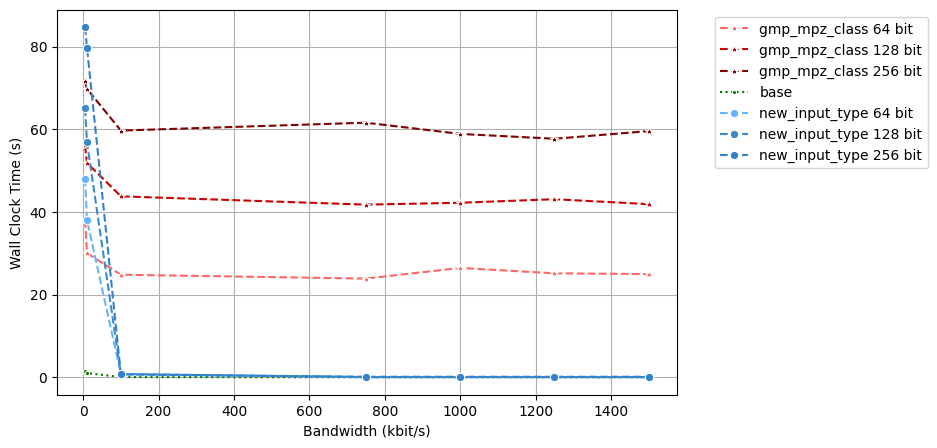
\includegraphics[width=0.8\textwidth]{plots/plots/online/wct_bandwidth_read_online.png}
    \caption{Online: Reading for increasing bandwidth, constant latency, and constant number of elements retrieved.
    The green curve is the base implementation by Vadapalli et al. 
    Red curves represent \textit{gmp\_mpz\_class}.
    The darker the red, the greater the entry size.
    \textit{128 bit}, for example, implies entry sizes of up to 128 bit.
    The blue curve represents \textit{new\_input\_type}.
    }
    \label{fig:readIncBandwidthOnline}
\end{figure}

\begin{figure}
    \centering
    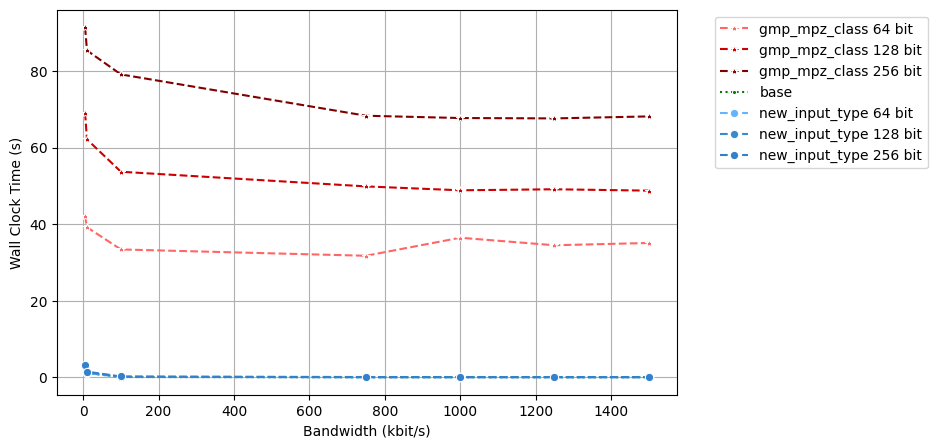
\includegraphics[width=0.8\textwidth]{plots/plots/online/wct_bandwidth_update_online.png}
    \caption{Online updating for increasing bandwidth, constant latency, and constant number of elements updated.
    The green curve is the base implementation by Vadapalli et al. 
    Red curves represent \textit{gmp\_mpz\_class}.
    The darker the red, the greater the entry size.
    \textit{128 bit}, for example, implies entry sizes of up to 128 bit.
    The blue curve represents \textit{new\_input\_type}.
    }
    \label{fig:updIncBandwidthOnline}
\end{figure}

\begin{figure}
    \centering 
    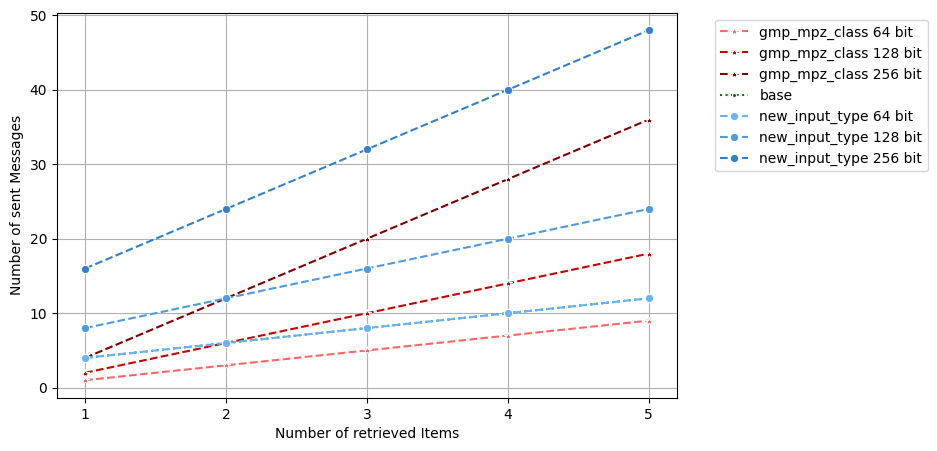
\includegraphics[width=0.8\textwidth]{plots/plots/online/message_num_read_online.png}
    \caption{Online: Number of messages sent for retrieving an increasing number of elements of constant depth.
    The green curve is the base implementation by Vadapalli et al. 
    Red curves represent \textit{gmp\_mpz\_class}.
    The darker the red, the greater the entry size.
    \textit{128 bit}, for example, implies entry sizes of up to 128 bit.
    The blue curve represents \textit{new\_input\_type}.
    }
    \label{fig:readMsgSentOnline}
\end{figure}

\begin{figure}
    \centering
    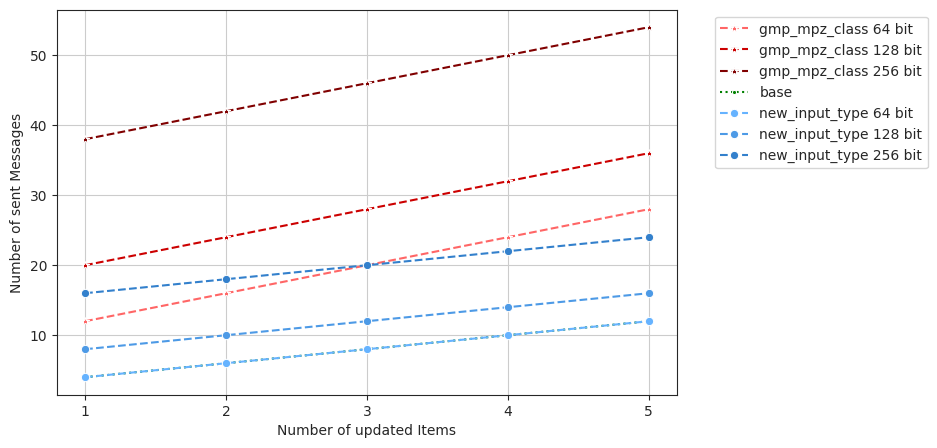
\includegraphics[width=0.8\textwidth]{plots/plots/online/message_num_update_online.png}
    \caption{Online: Number of messages sent for updating an increasing number of elements of constant depth.
    The green curve is the base implementation by Vadapalli et al. 
    Red curves represent \textit{gmp\_mpz\_class}.
    The darker the red, the greater the entry size.
    \textit{128 bit}, for example, implies entry sizes of up to 128 bit.
    The blue curve represents \textit{new\_input\_type}.
    }
    \label{fig:updMsgSentOnline}
\end{figure}